\documentclass{article}

% Language setting
% Replace `english' with e.g. `spanish' to change the document language
\usepackage[english]{babel}

% Set page size and margins
% Replace `letterpaper' with `a4paper' for UK/EU standard size
\usepackage[letterpaper,top=2cm,bottom=2cm,left=3cm,right=3cm,marginparwidth=1.75cm]{geometry}

% Useful packages
\usepackage{amsmath}
\usepackage{graphicx}
\usepackage[colorlinks=true, allcolors=blue]{hyperref}
\usepackage{booktabs}
\usepackage{cleveref}

\title{Innovation fond notes}
\author{Tue Herlau}

\begin{document}
\maketitle

% \begin{abstract}
% Your abstract.
% \end{abstract}

\section{Introduction}
The application deals with the situation where a user want to solve different computer vision tasks based on videos. 

\subsection{Problem identification}
As I see it, these are the main characteristics of the problem: 

\subsubsection{Tasks variability}
We imagine thedre are many, different tasks such as
\begin{itemize}
    \item Detection of objects
    \item Counting 
    \item Binary labelling
    \item Continuous measurements/estimation 
    \item Outlier detection
\end{itemize}
The tasks are imagined to be of greatly varying complexity, so that some (if a door is open or closed in a well lit environment) can be solved by simply consider pixel intensities while other, such as counting unusual objects, are open ended and fundamentally quite difficult. A prototypical example of input data is one where a user has mounted a camera to oversee a conveyor belt with pastries.

\subsubsection{Continuity}
Some applications, such as counting the number of different people on a building site during a way, would seem to involve integration of temporal information (tracking). It is in general probably worth distinguishing between what the visual model outputs, and how these are transformed into metrics the users are interested in. 
As an example, the user could be interested in the rate in which pastries are produced rather than the raw counts.

\subsubsection{Automated task selection}
Secondly, given an input video stream, the system should require an minimum amount of setup. Specifically it should not rely on manual labelling of images by the user. As an example, suppose the user want to count pastries on a conveyor belt. This is imagined to work as follows:
\begin{itemize}
    \item The user select 'count objects' from a dropdown box
    \item The system ideally understands that the relevant object to count is the pastries
\end{itemize}

\subsubsection{Task ambiguity} 
The automated workflow should be balanced against the natural demand that most videos will contain several ambiguous tasks. For instance, the user could be interested in counting the number of people who pass behind the conveyor belt rather than the number of pastries, or how many pastries are missing glazing rather than the total number of pastries.

\section{Defining the problem}
A task is here thought to be composed of 
\begin{itemize}
    \item A \emph{task type} (e.g., counting), written as $t$
    \item A \emph{specified task}, which is a task type with the additional context which specify the task exactly (e.g., counting humans)
\end{itemize}
Let $x$ the input data (e.g. a short segment of video) and $c$ a customer. The specified task will therefore be written a $t(x)$. The output of the model will be written as $y$; it may be relevant to distinguish between different output modalities (numbers, binary labels, classes, etc.) but for now I will just stick with $y$. The system therefore produce outputs:
$$
p(y \mid t, x) = p(y \mid t(x)).
$$
Automated task selection therefore means that we produce an output without having a specific task, e.g. there is a decision mechanism $d$ that allows us to define: 
$$
p(y \mid x) = p(y \mid t(x)), \quad t = d(x, c).
$$

Lets consider the pastries example. In this case $t$ could be counting. So lets assume:
$$
t = \texttt{count}
$$
it is possible that just given this task, it is possible to define rules that identifies that the pastries is the relevant thing to count (i.e., object detection + what changes between images), i.e. that $t(x, c)$ corresponds to pastry-counting. However, this approach would not work if we wanted to count non-glazed pastries, and it is easy to imagine that outside the most stereotypical situations the approach would fail (include erroneous objects or exclude objects we were interested in). 




\section{Architectural ideas}


\subsection{Plug-in architecture}
One approach is to build a general plug-in container and a number of different plug-ins. Then, for a given input image, return the value from the relevant estimator (determined by the user prompt or from a palette of inputs). The plug-ins can be hardcoded or trained.

I would consider this as the default way to build the vision system, and it is worth reflecting on the advantages and disadvantages:

\begin{center}
\begin{tabular}{|p{.45\linewidth}|p{.45\linewidth}|}
\hline
\textbf{Pros} & \textbf{Cons} \\
\hline
\begin{itemize}
    \item If it works it really works -- great out-of-the-box results
    \item Allows the system to do something correctly from day 1
    \item Could sell special plugins to (big) customers    
\end{itemize} &
\begin{itemize}
    \item When it does not work, it really does not work
    \item New task = new plugin
    \item Kind of defeat the idea of a central site with all information    
    \item Maintain/update plugins while avoiding regression
\end{itemize} \\
\hline
\end{tabular}
\end{center}
One of my concerns with the plug-in system is purely technical. Lets say we can define a plugin that figures out on its own that it should count pastries, and now we want to modify the plugin to count the rate at which pastries are produced. This involves a lot of overlap in functionality.  I think I have two main concerns:

\begin{itemize}
\item Interdependence between different plug-ins: If the plug-ins are independent, it would (perhaps?) involve quite a lot of duplicated effort (object detection, segmentation, labelling, etc.). If they depend on a library (e.g. for performing segmentation), would this risk the possibility of a lot of regression when this pipeline is altered, causing existing customer pipelines fail. In other words, this seem like a system that can easily acrue a lot of technical debt. 
\item Brittle: If a plug-in almost-but-not-quite work (a plug-in counts the bottles in the wending machine but unfortunately include snacks in the count by a mistake) it is a bit tough to go tell the customer to pound sand and hire a consultant. It would be useful to know  how frequent this situation is expected to occur, perhaps by comparing against how smooth existing solution works out of the box. 
\end{itemize}


\begin{figure}[t]
    \centering
    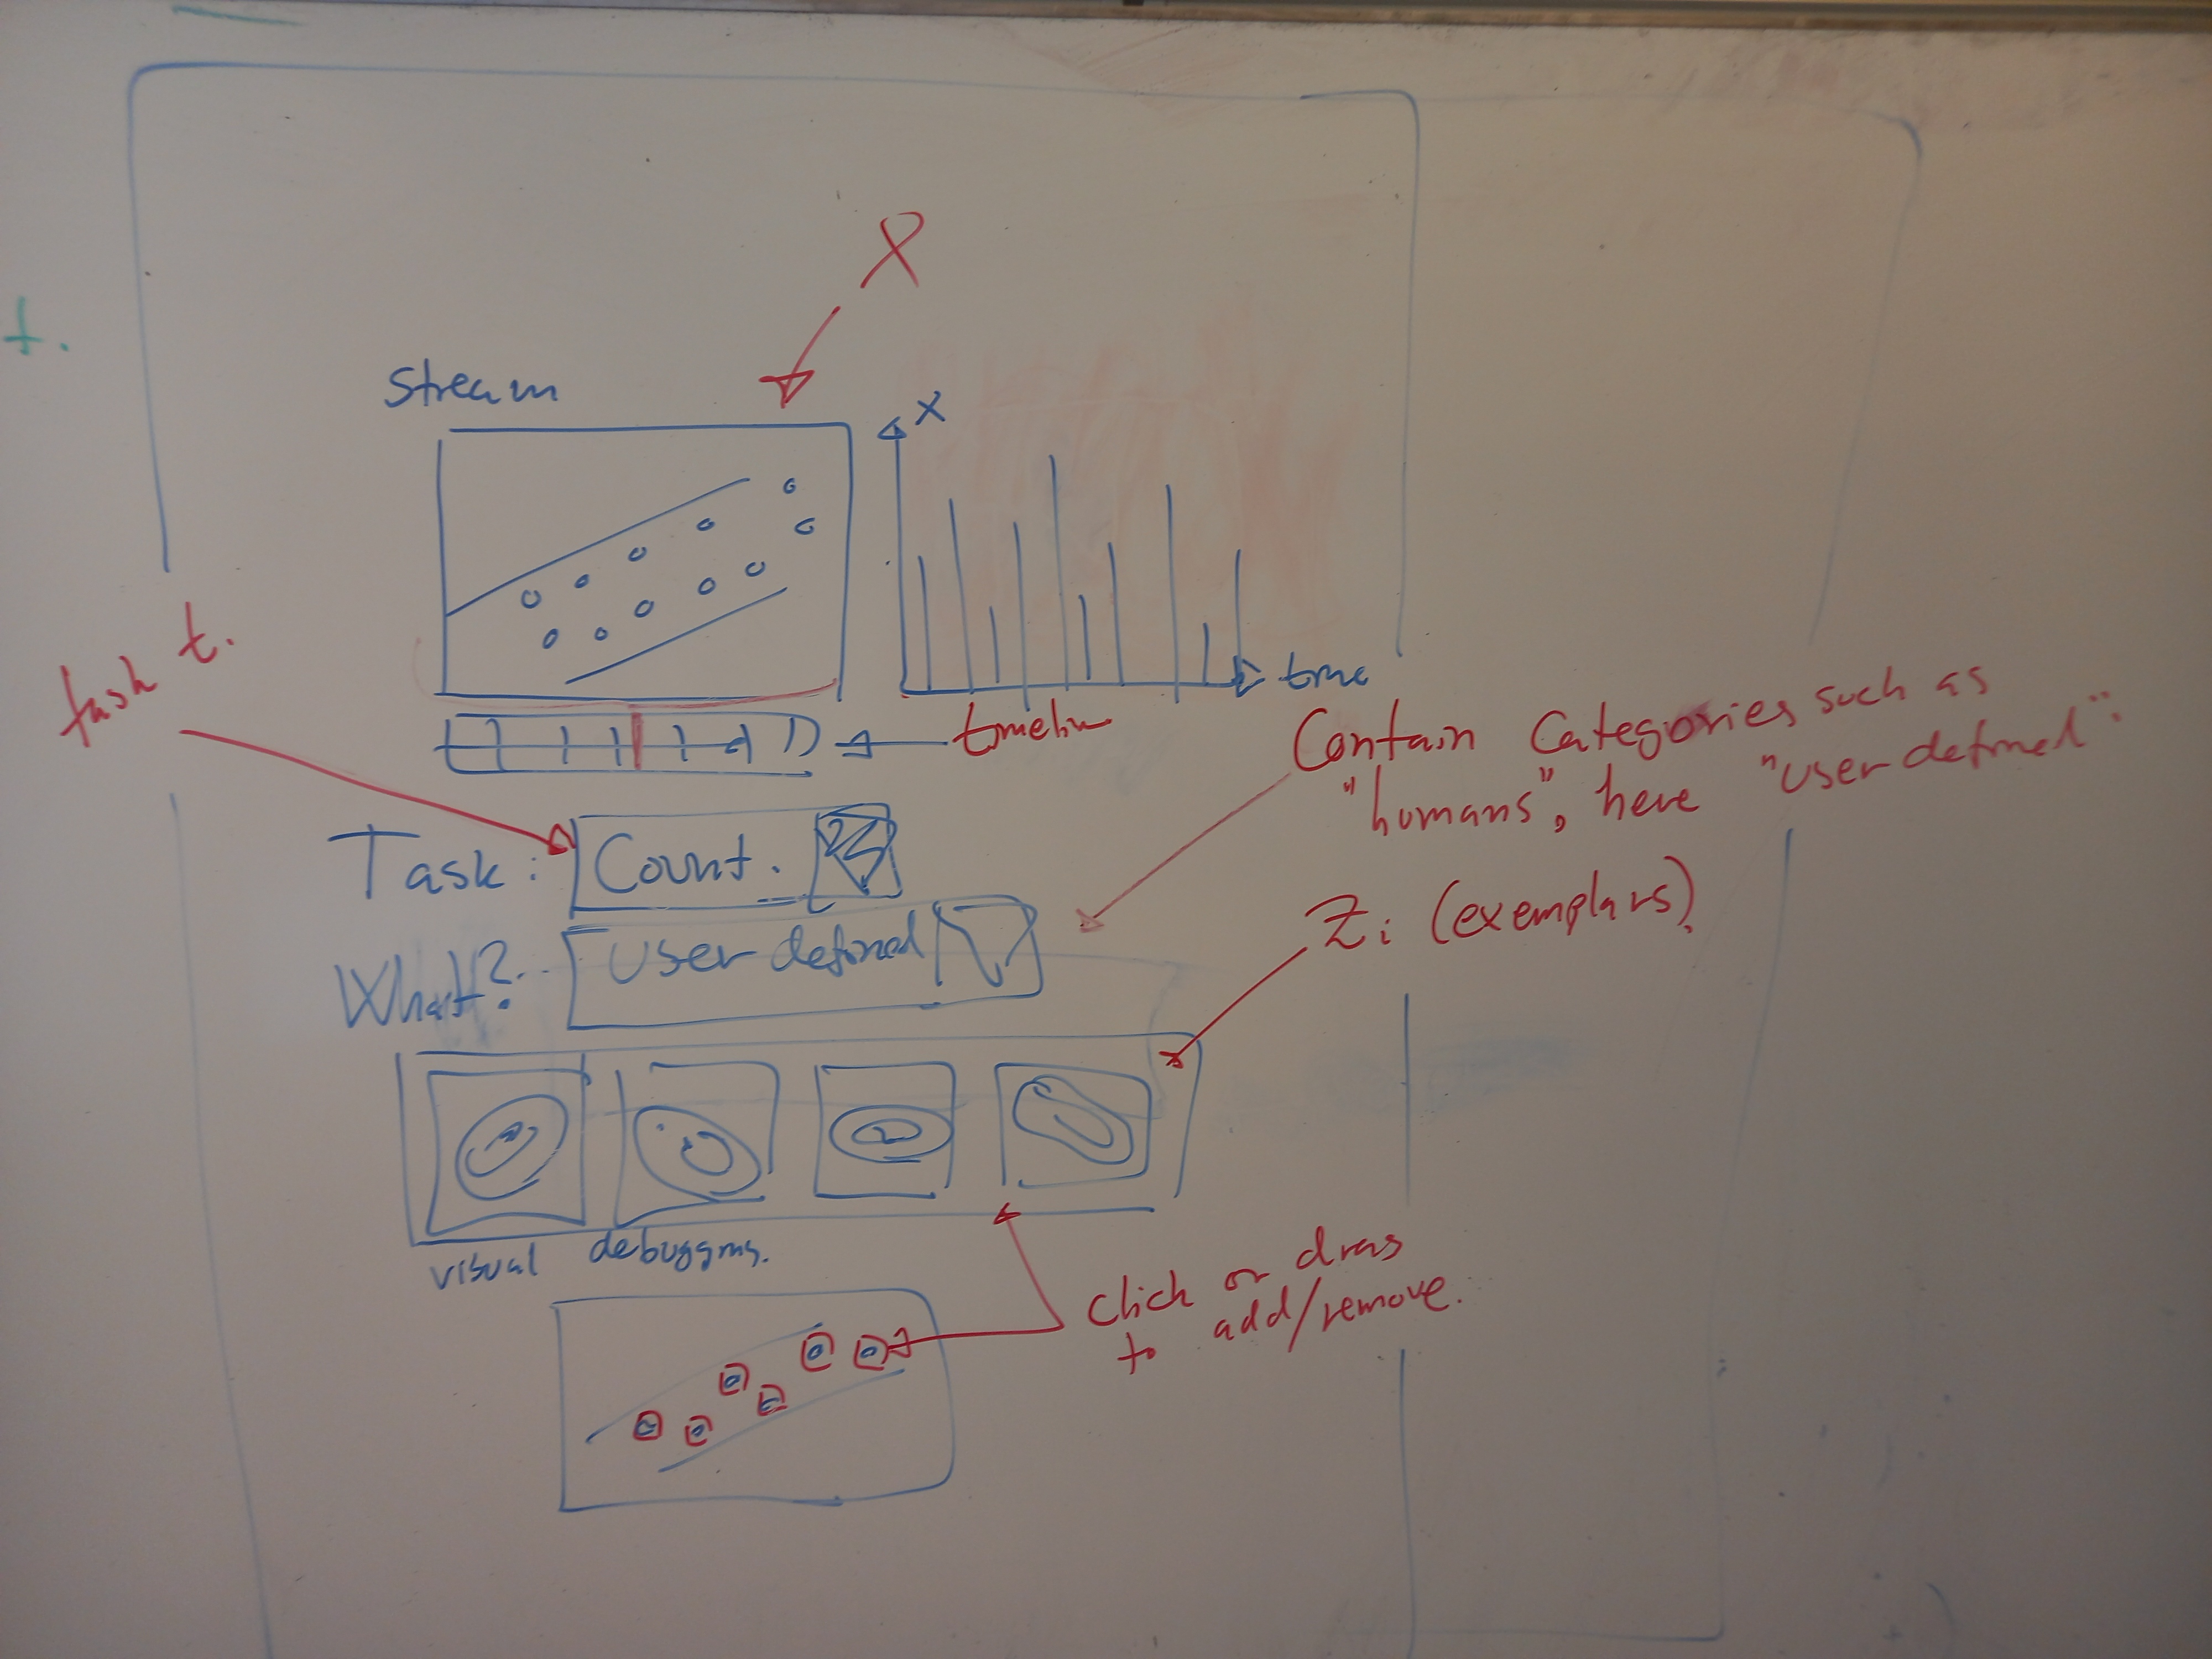
\includegraphics[width=\linewidth]{20230420_104629.jpg}
    \caption{A counting example. The method maintain (and show) candidate images that are counted $z_i$ to allow visual debugging/correction. }
    \label{fig1}
\end{figure}

\subsection{Transformer architecture}
Transformer-based large language models (LLMs) can perform operations on text that seem analogous to what we hope to do. For instance:
\begin{itemize}
    \item Produce widely divergent outputs based on the same input data and different (but near identical) prompts
    \item Identify and use salient properties of input data (the transformer attention mechanism)
    \item Exhibit limited emergent properties (generalization to adjacent but novel tasks)
    \item Exhibit near-but-non-human intelligence on limited task domains.
\end{itemize}
Since the prompt will often involve visual elements (\texttt{count pastries}), it will probably be useful to consider the prompt as comprised of:
\begin{itemize}
    \item A list of exemplar images relevant to the query (e.g., images of pastries), $z_1,z_2,\dots$
    \item A one-hot vector encoding the task type (or more generally, a LLM vector representation of an input query)    
\end{itemize}
The exemplar images will be encoded by another transformer to give vector representations $h(z_1), h(z_2), \dots$ and combined (using e.g. hierarchical convolutions) to a single vector $\textbf z =h(z_1,\dots,z_n)$. During inference, this representation is fed into the decoder layer; this means that for each patch in the vision transformer, it will have access to both a vector representation of that patch, and a vector representation of what it should count, and hence counting becomes somewhat analogous to vector lookup. Inference for a given task is thus comprised of:
\begin{itemize}
    \item Select overall task type (e.g. discrete counting)
    \item Let e.g. an object detector or some other heuristic determine the objects to count, $z_1,\dots$, or allow the user to select them manually. The interface should give feedback on what is being counted. 
    \item Produce output using the transformer $y = T(x, \textbf z = h(z_1,\dots,), t, c)$
\end{itemize}
see \cref{fig1}. Normal training can proceed in three modes:
\begin{itemize}
    \item During a fairly frequent online mode (user-invoked) where the first many layers, including the embedding $h$, is kept fixed and only the last output layers are updated to adapt to a specific company relevant task. 
    \item During offline training where both the transformer and embedding is trained jointly
    \item Thirdly, by training the extraction process of the image patches itself; the simplest version would simply be a binary labelling which for each candidate context image $z_i$, frame $x$, and task $t$ determines the probability that $z_i$ should be included or not:
    $$
    p(\textrm{include} = \textrm{True}/\textrm{False} \mid x, c, t)
    $$
(the candidate images would be obtained using a standard image segmentation method, or based on those candidates users had previously rejected).
\end{itemize} 

\subsection{InstructGPT}
InstructGPT is by many considered one of the reasons for ChatGPTs success. InstructGPT works by using another neural network to determine (predict) the quality of an output as judged by a human; this had three main benefits: (1) Humans were able to give more relevant input; i.e. more human-like evaluations -- instead of saying 'this is what you should say', humans judged whether something chatGPT said was better or worse; this is an important distinction as we can often judge whether one thing is better than another even though we lack the skill or time to produce either inputs  (2) it allowed the system to train on unlabelled data (3) it gave a more robust system since humans would punish ideosyncratic behavior of the model (for instance, repeating sentences many times).

It would be interesting to include a similar scheme in this case: instead of giving specific input/output values (there are 320 cookies in the picture), humans would instead provide feedback on the quality (scale from 1-5) of the prediction, perhaps compared to another estimate. This comparison could for instance take into account whether the visual features the system focused on correlate with what we actually want to count.

\begin{center}
\begin{tabular}{|p{.45\linewidth}|p{.45\linewidth}|}
\hline
\textbf{Pros} & \textbf{Cons} \\
\hline
\begin{itemize}
    \item Potentially much more open-ended design; a system that gets better with more diverse tasks
    \item Attempt to build on architectures that have shown great potential in other domains
    \item Easier to put in headline form: \emph{"A ChatGPT for visual tasks"}. Better for the application?
\end{itemize} &
\begin{itemize}
    \item Higher risk; it could flat out just work really poorly
    \item Requires quite a lot of computational resources
    \item Visual debugging asides, the failure modes will ultimately be hard to attribute to a single thing (the neural network apparently did not work)
\end{itemize} \\
\hline
\end{tabular}
\end{center}


\bibliographystyle{alpha}
\bibliography{sample}

\end{document}